\newif\ifuptexmode\uptexmodefalse

\ifnum\jis"2121="3000

 %% for upLaTeX
 \documentclass{ujarticle}
 \def\pLaTeXorupLaTeX{upLaTeX}
 \uptexmodetrue
 \def\innerencoding{UPTEX}
 \def\tounicode{pdf:tounicode UTF8-UCS2}

\else

 %% for pLaTeX
 \documentclass{jarticle}
 \def\pLaTeXorupLaTeX{pLaTeX}
 \uptexmodefalse

 \ifnum\jis"2121="A1A1
  \def\innerencoding{EUC}
  \def\tounicode{pdf:tounicode EUC-UCS2}
 \fi
 \ifnum\jis"2121="8140
  \def\innerencoding{SJIS}
  \def\tounicode{pdf:tounicode 90ms-RKSJ-UCS2}
 \fi

\fi

\usepackage{graphicx}

%%%%%%%%
% hyperref $B4XO"$N@)8f$r%3%^%s%I%i%$%s$+$i9T$&(B
% (1),(2),(3) $B$N$I$l$+$r<B9T$9$l$P$h$$!#(B
%   (1) $B2?$b$7$J$$(B
%   $ uplatex bkmk-jis.tex
%   (2) hyperref + dvipdfmx
%   $ uplatex "\def\withhyperref{dvipdfmx}\input" bkmk-jis.tex
%   (3) hyperref + dvips + modified convert-euc.txt + distiller/ps2pdf
%       hyperref + dvips + convbkmk.rb + distiller/ps2pdf
%   $ uplatex "\def\withhyperref{dvips}\input" bkmk-jis.tex
%%%%%%
\makeatletter
\def\@dvipdfmx{dvipdfmx}
\def\@dvips{dvips}

\ifx\withhyperref\@undefined
 \def\withhyperref{undefined}
\else

\ifx\withhyperref\@dvipdfmx
 \def\@hyperrefkeyval{dvipdfm}
\fi
\ifx\withhyperref\@dvips
 \def\@hyperrefkeyval{dvips}
\fi

\usepackage[\@hyperrefkeyval,%
bookmarks=true,%
bookmarksnumbered=true,%
bookmarkstype=toc,%
%pdfstartview={FitBH -32768},%
pdftitle={$B$$$m$$$m3N$+$a$F$_$k(B},%
pdfsubject={hyperref$BJT(B},%
pdfauthor={$BL>L5(B $B8"J<1R(B},%
pdfkeywords={TeX; dvips; dvipdfmx; bookmark; hyperref; $B$7$*$j(B; pdf}%
]{hyperref}

\fi

\ifx\withhyperref\@dvipdfmx
 \AtBeginDvi{\special{\tounicode}}
\fi

\makeatother

\title{$B$$$m$$$m3N$+$a$F$_$k(B}

\author{$BL>L5(B $B8"J<1R(B}

\oddsidemargin0mm
\evensidemargin0mm
\topmargin-15mm
\textwidth162mm
\textheight245mm

\begin{document}
\maketitle
\section{section title by ASCII}
test test.

hyperref with: \withhyperref
\typeout{### hyperref with: \withhyperref}

pLaTeX or upLaTeX: \pLaTeXorupLaTeX
\typeout{### pLaTeX or upLaTeX: \pLaTeXorupLaTeX}

inner encoding: \innerencoding
\typeout{### inner encoding: \innerencoding}

\begin{figure}
 \begin{center}
  \scalebox{0.2}{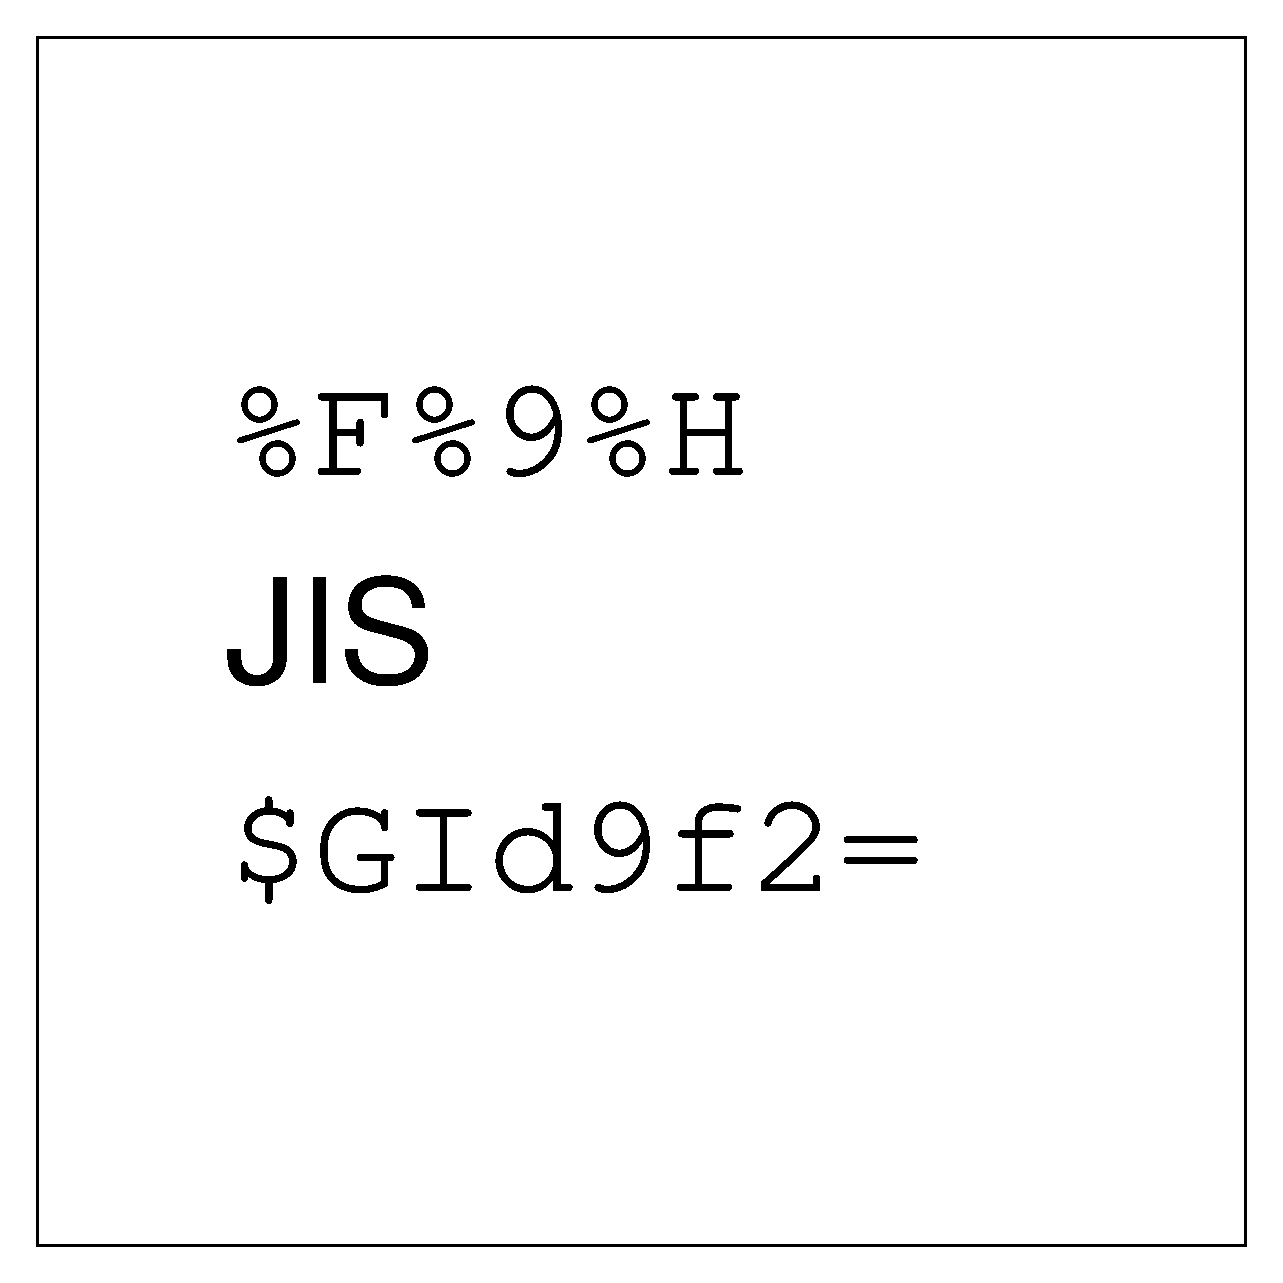
\includegraphics{box-jis.eps}}
  \caption{JIS$B$GId9f2=$5$l$?(BEPS$B%U%!%$%k(B}
  \label{fig:box-jis}
 \end{center}
\end{figure}
%\begin{figure}
% \begin{center}
%  \scalebox{0.2}{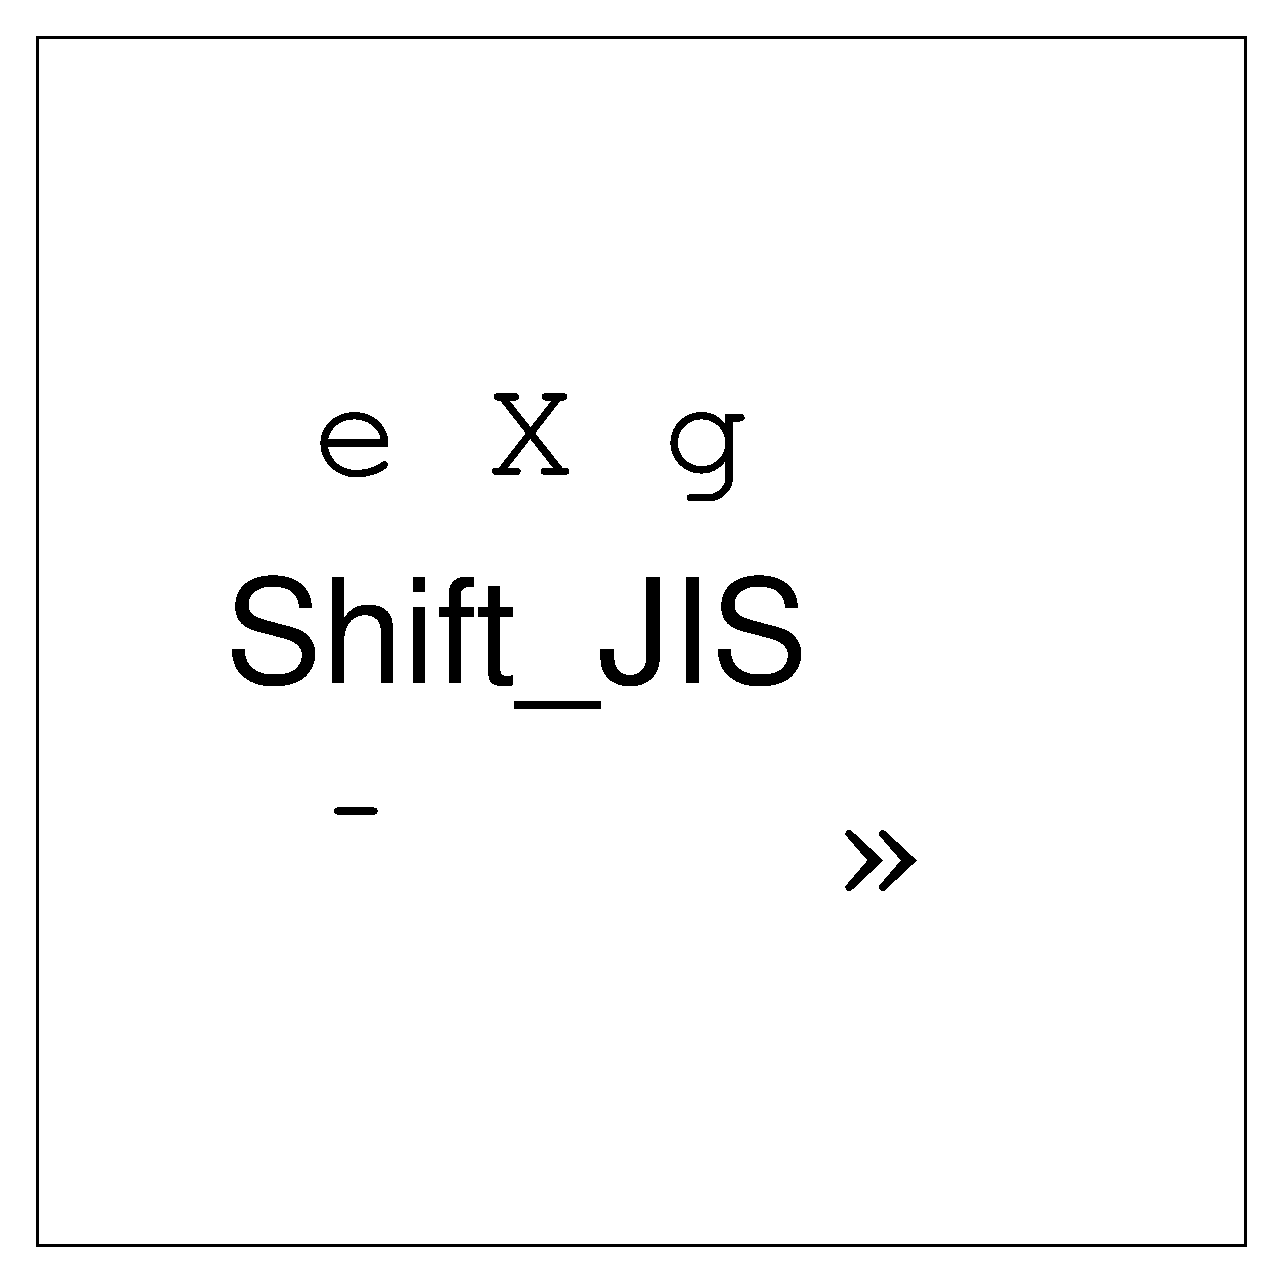
\includegraphics{box-sjis.eps}}
%  \caption{Shift\_JIS$B$GId9f2=$5$l$?(BEPS$B%U%!%$%k(B}
%  \label{fig:box-sjis}
% \end{center}
%\end{figure}
%\begin{figure}
% \begin{center}
%  \scalebox{0.2}{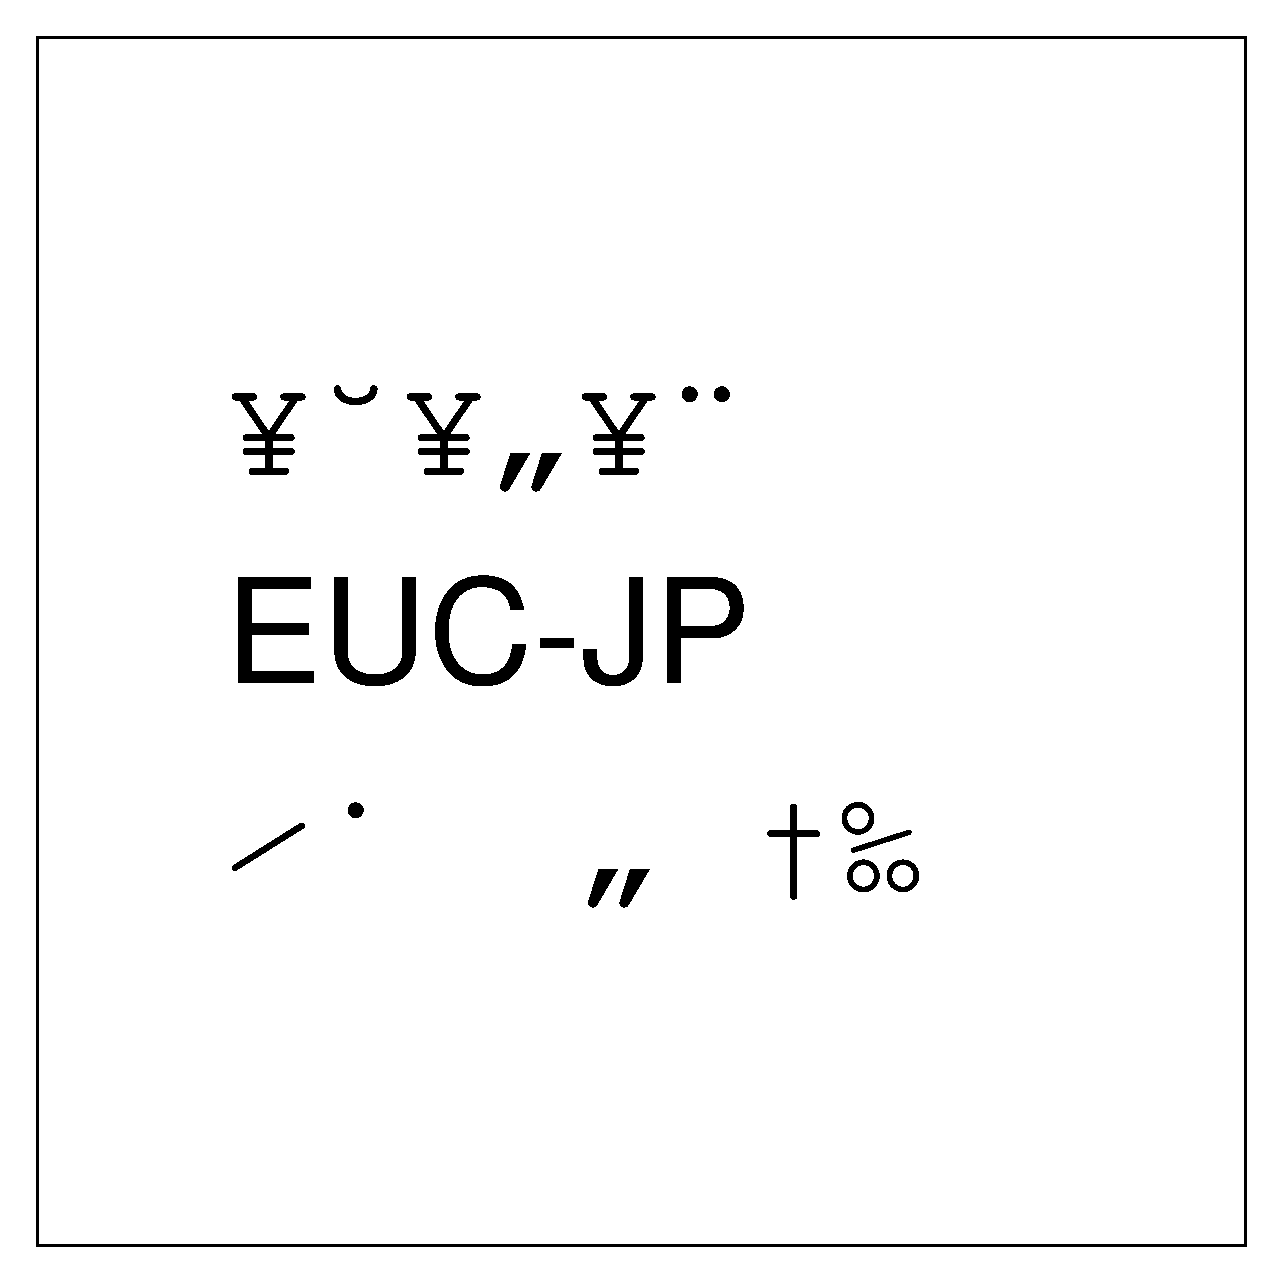
\includegraphics{box-euc.eps}}
%  \caption{EUC-JP$B$GId9f2=$5$l$?(BEPS$B%U%!%$%k(B}
%  \label{fig:box-euc}
% \end{center}
%\end{figure}
%\begin{figure}
% \begin{center}
%  \scalebox{0.2}{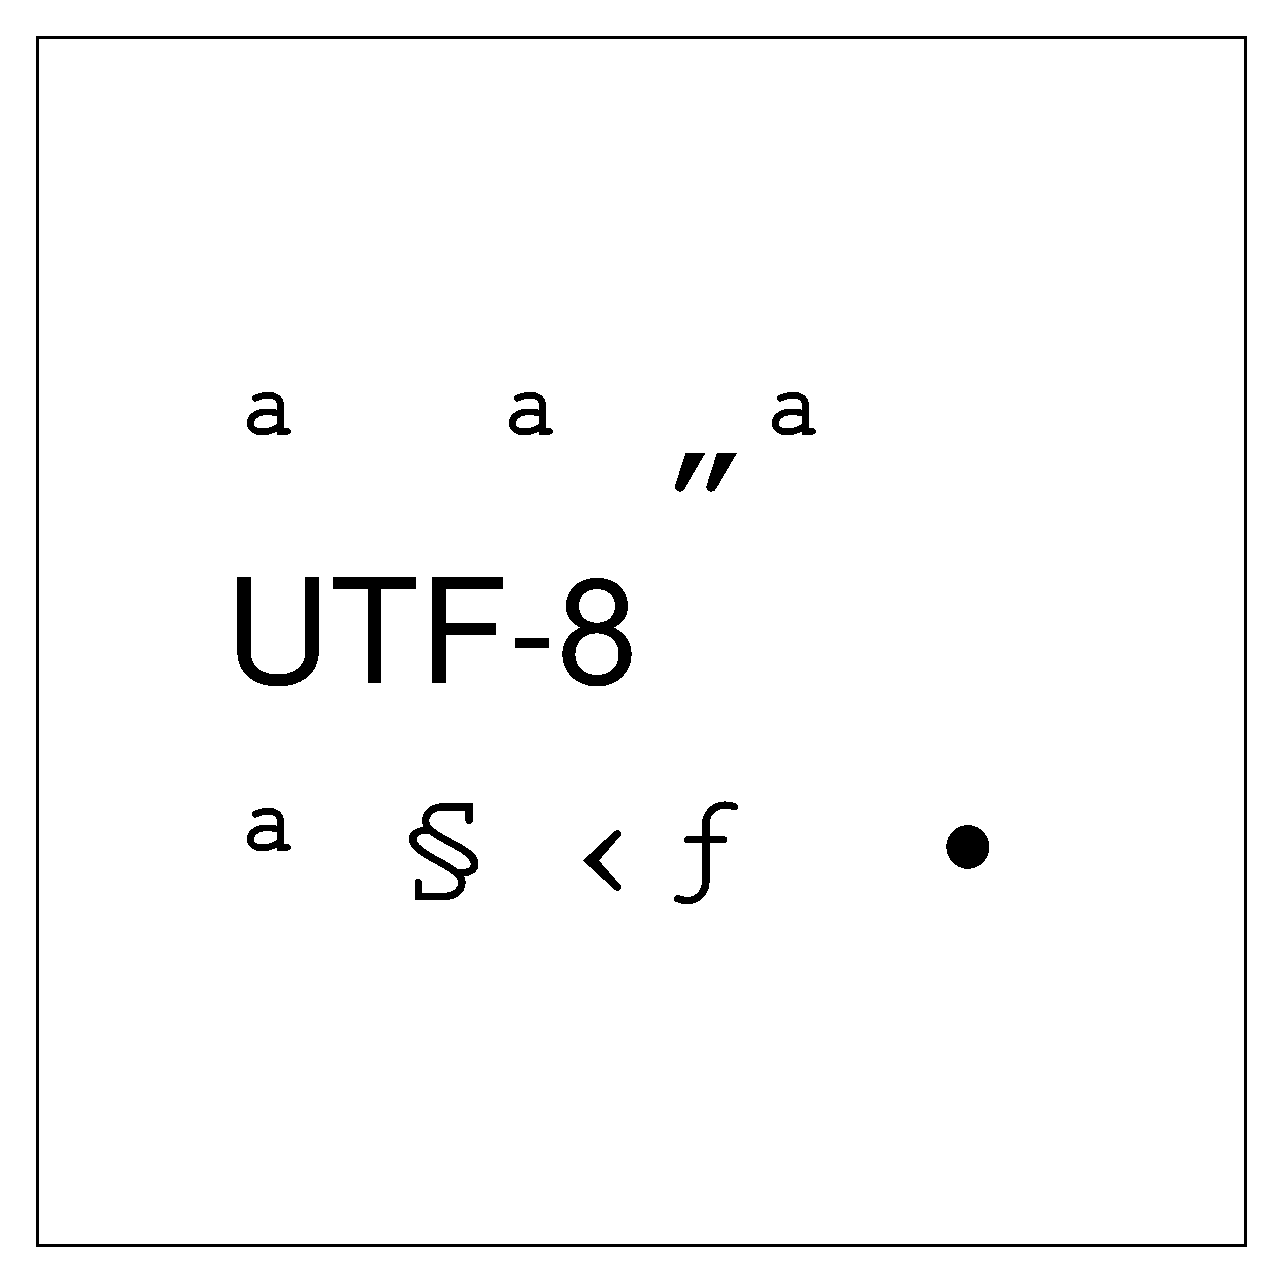
\includegraphics{box-utf8.eps}}
%  \caption{UTF-8$B$GId9f2=$5$l$?(BEPS$B%U%!%$%k(B}
%  \label{fig:box-utf8}
% \end{center}
%\end{figure}
\section{$B&A&B&C(B}
test test.

\section{$B'Q'R'S(B}
test test.

\section{$B%;%/%7%g%s(B}
test test.
\subsection{$B%5%V%;%/%7%g%s(B($B3g8L(B)}
test test.

\end{document}
